%! vim: spl=cs:
\documentclass[a0paper,portrait,fontscale=.25]{baposter}

\usepackage{relsize}
\usepackage[utf8]{inputenc}
\usepackage{PTSans}
\renewcommand{\familydefault}{\sfdefault}

\begin{document}

\background{%
%\includegraphics{paticky_tisk_up_01.pdf}
}

\def\bp{\parindent0pt\parskip=\smallskipamount}
\definecolor{main}{cmyk}{0.06,0.26,0.91,0}
\definecolor{other}{cmyk}{0.94,0.74,0.09,0}

\def\alert#1{\textbf{\color{other}#1}}

\begin{poster}{
	grid=false,
	columns=6,
	background=user,
	borderColor=main,
	headerFontColor=other,
	headerColorOne=main,
	headerColorTwo=main!50!white,
	textborder=rectangle,
	headershape=roundedright,
%	headerborder=none,
%	boxColorOne=main,
%	boxColorTwo=main,
	headerfont=\Large\bfseries,
	headerborder=open,
	boxshade=none,
}
{ % Eyecatcher
}
{%
The Chicken-and-Egg Problem of Landmark-Driven Molecular Dynamics: Are Random Landmarks Useful?
}
{
\vrule height2ex width0pt Aleš Křenek, Jana Hozzová, Jaroslav Olha, Martin Kurečka, Dalibor Trapl, Vojtěch Spiwok
}
{ % logo
}

\headerbox{Metadynamics with Path Collective Variables}{name=pcv,column=0,row=0,span=3}{
\bp
Molecular dynamics of proteins can be guided to explore wider range of configurational space (folding paths in particular) with biased potential built on path collective variables, which are derived from a set of landmark structures which approximate the desired trajectory
[ \lower.9ex\hbox{
\includegraphics[height=2.8ex]{from-a-to-b}}
\lower.9ex\hbox{
\includegraphics[height=2.8ex]{meta-isomap}} ].
The technique can reduce the time of the MD simulation dramatically. On the other hand, the choice of landmarks is the core of the “chicken and egg” problem – if we know the landmarks along the trajectory, what would be the reason of recomputing the same trajectory? (Well, things are not so simple, but this is the core.)
}

\headerbox{Randomly Generated Landmarks}{name=vystupy,column=3,span=3}{
\bp
In this study, we aim at computing the trajectories de novo, without prior knowledge. First, a set of several hundreds to thousands of barely feasible landmarks is generated by random twisting of peptide bonds in the subject protein. Many such structures contain steric clashes and other unrealistic properties. Those are filtered by steepest descent energy minimization in vacuo, using simple force field (Amber99); if the minimization fails or it stops at too high energy, the structure is discarded. Typically, sufficiently high number (e.g. more than 80 \%) of the structures pass. 
}

\headerbox{}{name=bigpic,column=0,span=6,below=pcv}
{
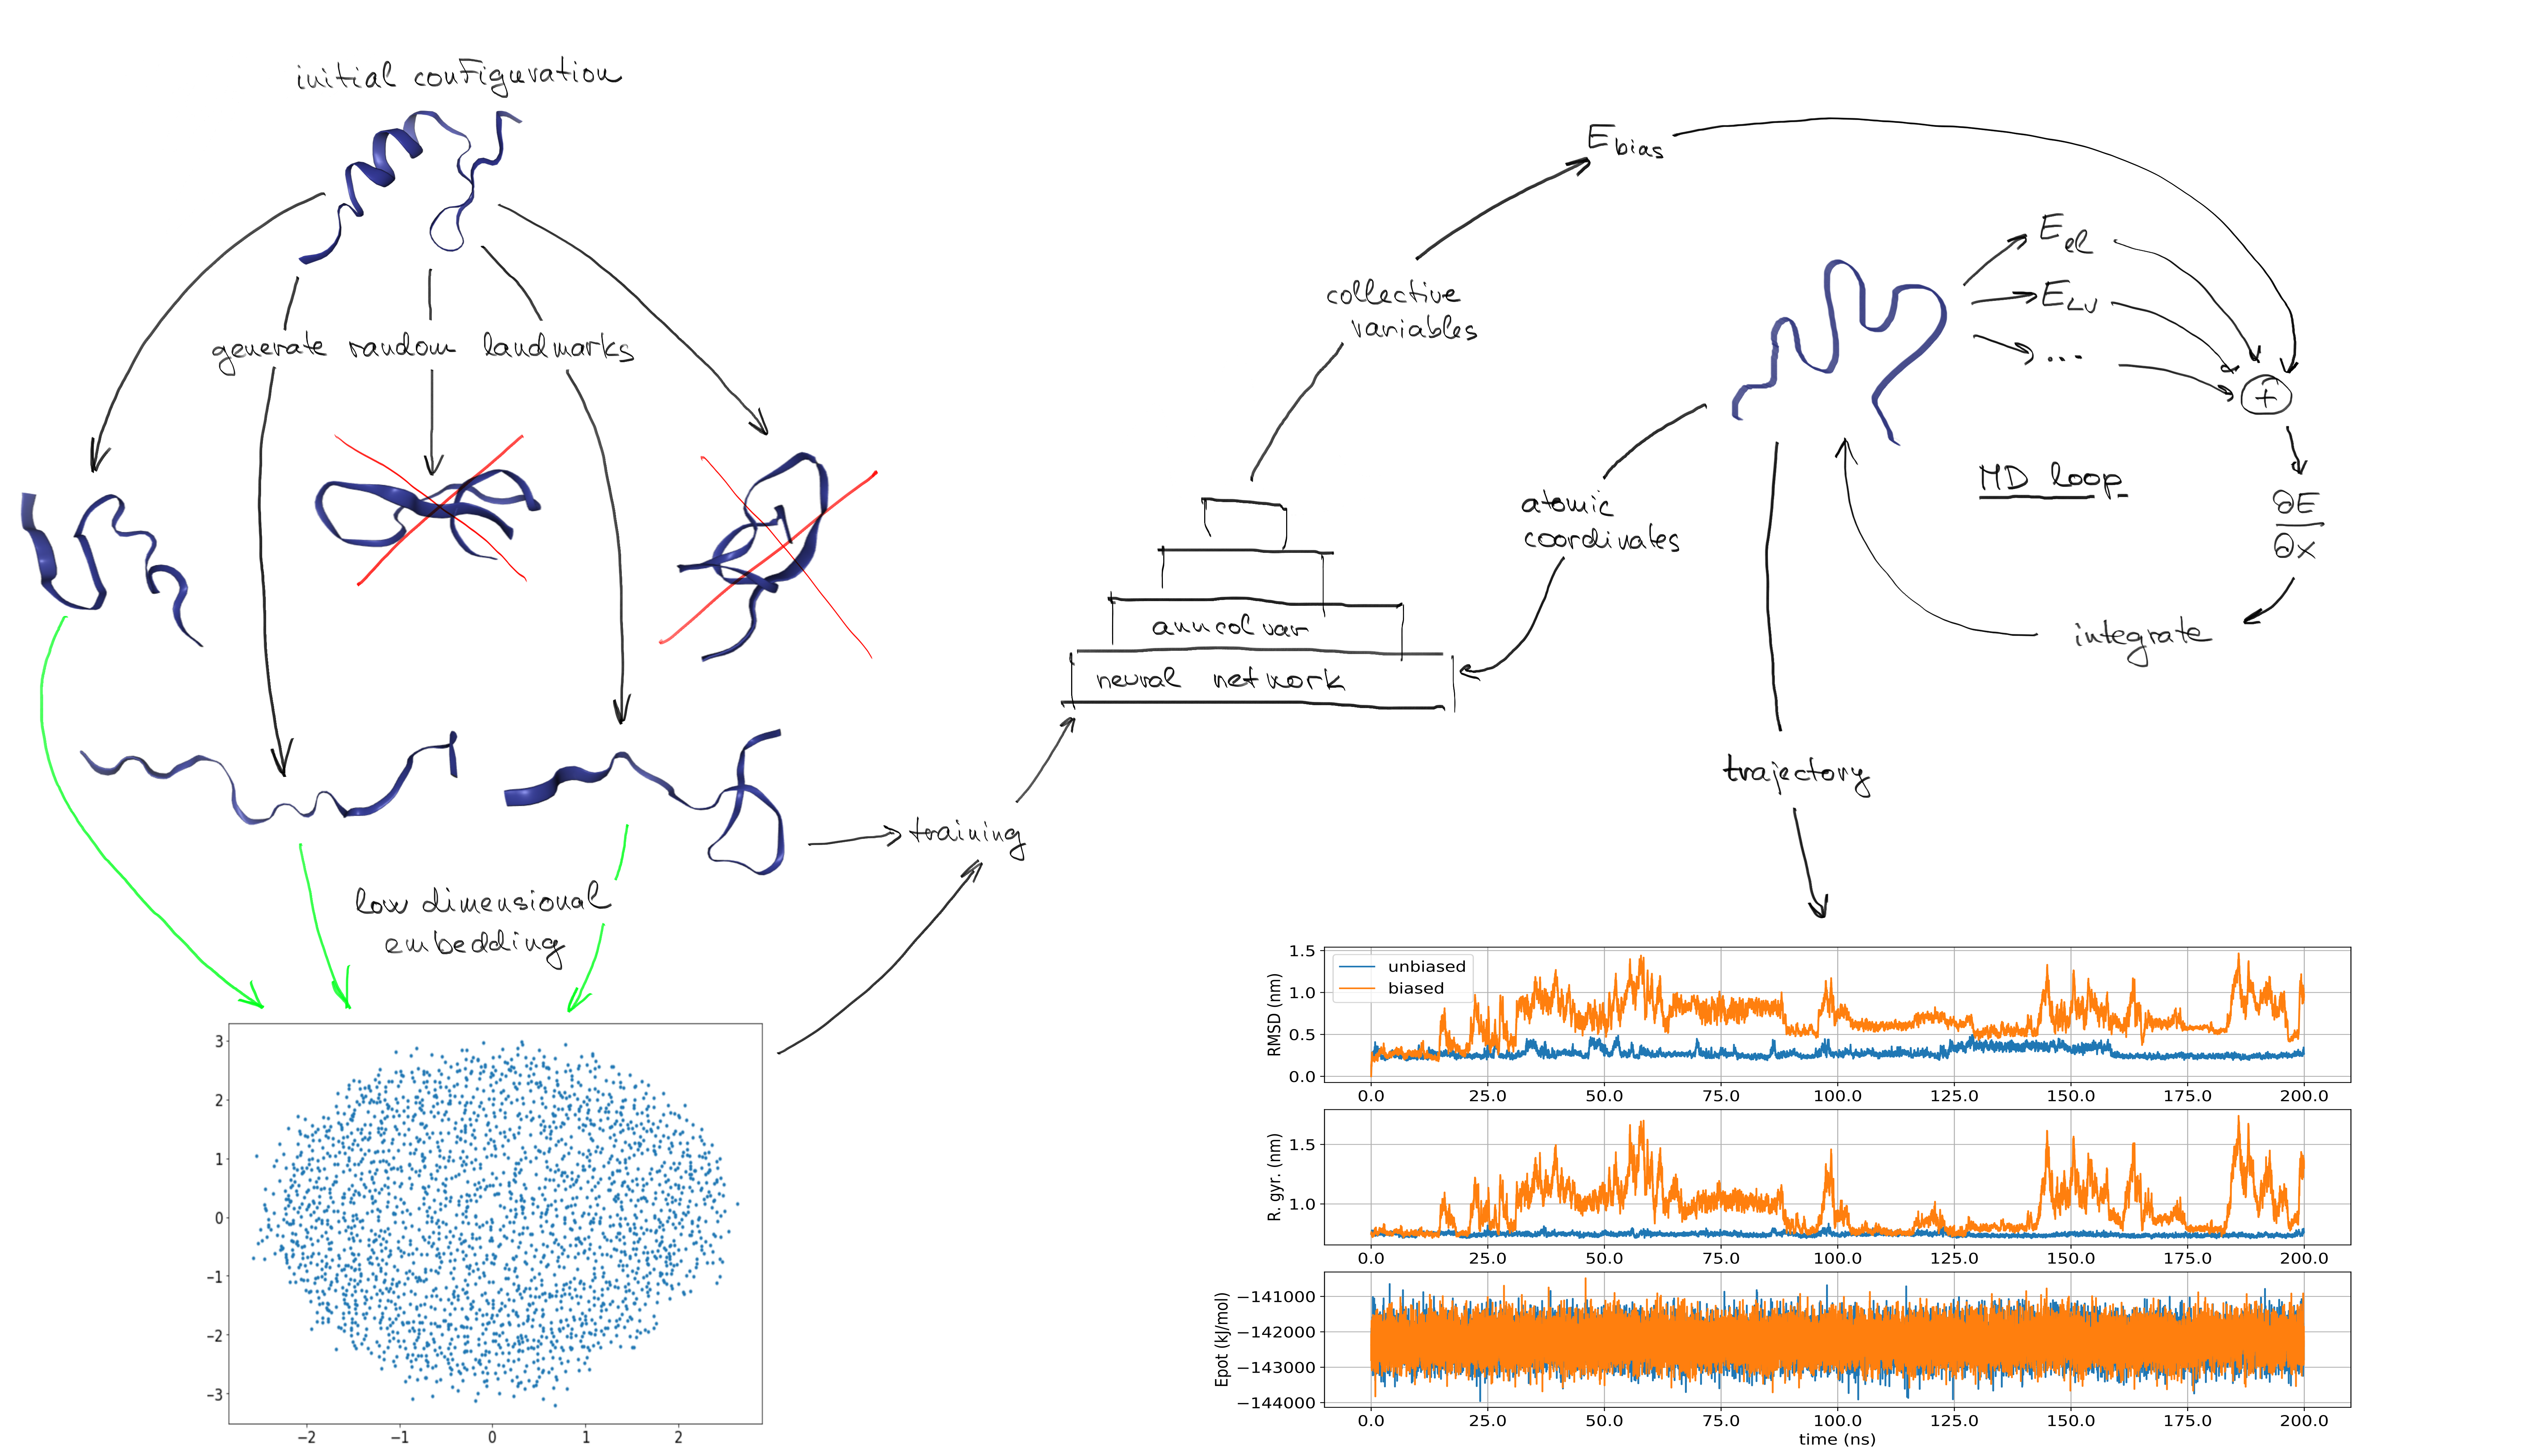
\includegraphics[width=\hsize]{bigpic2}
}

\headerbox{Implementation}{name=impl,column=0,below=bigpic,span=4}{
\bp
Lorem ipsum \dots
}

\headerbox{Acknowledgement}{name=ack,column=4,below=bigpic,span=2}{
\bp
GAČR
e-Infra
}

\end{poster}
\end{document}
